% This is the Amherst College LaTeX thesis template.
% See http://web.reed.edu/cis/help/latex.html for help. There are a
% great bunch of help pages there, with notes on
% getting started, bibtex, etc. Go there and read it if you're not
% already familiar with LaTeX.
%
% Any line that starts with a percent symbol is a comment.
% They won't show up in the document, and are useful for notes
% to yourself and explaining commands.
% Commenting also removes a line from the document;
% very handy for troubleshooting problems. -BTS

% As far as I know, this follows the requirements laid out in
% the 2002-2003 Senior Handbook. Ask a librarian to check the
% document before binding. -SN

%%
%% Preamble
%%
% \documentclass{<something>} must begin each LaTeX document
\documentclass[12pt,twoside]{amherstthesis}
% Packages are extensions to the basic LaTeX functions. Whatever you
% want to typeset, there is probably a package out there for it.
% Chemistry (chemtex), screenplays, you name it.
% Check out CTAN to see: http://www.ctan.org/
%%
\usepackage{graphicx,latexsym}
\usepackage{amsmath}
\usepackage{amssymb,amsthm}
\usepackage{longtable,booktabs,setspace}
\usepackage{chemarr} %% Useful for one reaction arrow, useless if you're not a chem major
\usepackage{rotating}

% Modified by CII
\usepackage[hyphens]{url}
\usepackage{hyperref}
\usepackage{lmodern}

% Added by CII (Thanks, Hadley!)
% Use ref for internal links
\renewcommand{\hyperref}[2][???]{\autoref{#1}}
\def\chapterautorefname{Chapter}
\def\sectionautorefname{Section}
\def\subsectionautorefname{Subsection}

\usepackage{caption}
\captionsetup{width=5in}

% \usepackage{times} % other fonts are available like times, bookman, charter, palatino

\title{My Comprehensive Evaluation}
\author{Kaitlyn E. Haase}
% The month and year that you submit your FINAL draft TO THE LIBRARY (May or December)
\date{February 26 2019}
\division{Statistics}
\advisor{Advisor A. Wagaman}
%If you have two advisors for some reason, you can use the following
%\altadvisor{Your Other Advisor}
%%% Remember to use the correct department!
\department{Mathematics and Statistics}
% if you're writing a thesis in an interdisciplinary major,
% uncomment the line below and change the text as appropriate.
% check the Senior Handbook if unsure.
%\thedivisionof{The Established Interdisciplinary Committee for}
% if you want the approval page to say "Approved for the Committee",
% uncomment the next line
%\approvedforthe{Committee}

% Below added by CII

%%% Copied from knitr
%% maxwidth is the original width if it's less than linewidth
%% otherwise use linewidth (to make sure the graphics do not exceed the margin)
\makeatletter
\def\maxwidth{ %
  \ifdim\Gin@nat@width>\linewidth
    \linewidth
  \else
    \Gin@nat@width
  \fi
}
\makeatother

\renewcommand{\contentsname}{Table of Contents}

\setlength{\parskip}{0pt}

\providecommand{\tightlist}{%
  \setlength{\itemsep}{0pt}\setlength{\parskip}{0pt}}

\Acknowledgements{
I want to thank my family.
}

\Dedication{

}

\Preface{

}

\Abstract{
In recent years, the amount of geographic data has increased immensely.
With new technology, the accuracy and complexity of data has also
improved. This has provoked statisticians to create techniques to best
analyze and draw conclusions from this new-found data. Earlier
techniques of spatial data were not equipped to handle the complexity
and quantity of the data. This project first explores how and why we
analyze data based on geographic information. Next, I will explain some
of the newer spatial data algorithms, including PAM (Partitioning Around
Medoids), CLARA (Clustering LARge Applications), and CLARANS (Clustering
Large Applications based on RANdomized Search). Example data will be
used to demonstrate CLARA, and the project will conclude a model to
predict cluster.
}


%%
%% End Preamble
%%
%

\begin{document}

      \maketitle
  
  \frontmatter % this stuff will be roman-numbered
  \pagestyle{empty} % this removes page numbers from the frontmatter

      \begin{acknowledgements}
      I want to thank my family.
    \end{acknowledgements}
  
  
  % Add table of abbreviations?

      \hypersetup{linkcolor=black}
    \setcounter{tocdepth}{2}
    \tableofcontents
  
      \listoftables
  
      \listoffigures
  
      \begin{abstract}
      In recent years, the amount of geographic data has increased immensely.
      With new technology, the accuracy and complexity of data has also
      improved. This has provoked statisticians to create techniques to best
      analyze and draw conclusions from this new-found data. Earlier
      techniques of spatial data were not equipped to handle the complexity
      and quantity of the data. This project first explores how and why we
      analyze data based on geographic information. Next, I will explain some
      of the newer spatial data algorithms, including PAM (Partitioning Around
      Medoids), CLARA (Clustering LARge Applications), and CLARANS (Clustering
      Large Applications based on RANdomized Search). Example data will be
      used to demonstrate CLARA, and the project will conclude a model to
      predict cluster.
    \end{abstract}
  
  
  \mainmatter % here the regular arabic numbering starts
  \pagestyle{fancyplain} % turns page numbering back on

  In recent years, the amount of geographic data has increased immensely.
  With new technology, the accuracy and complexity of data has also
  improved. This has provoked statisticians to create techniques to best
  analyze and draw conclusions from this new-found data. Earlier
  techniques of spatial data were not equipped to handle the complexity
  and quantity of the data. This project first explores how and why we
  analyze data based on geographic information. Next, I will explain some
  of the newer spatial data algorithms, including PAM (Partitioning Around
  Medoids), CLARA (Clustering LARge Applications), and CLARANS (Clustering
  Large Applications based on RANdomized Search). Example data will be
  used to demonstrate CLARA, and the project will conclude a model to
  predict cluster.
  
  \onehalfspacing
  
  \chapter*{Introduction}\label{introduction}
  \addcontentsline{toc}{chapter}{Introduction}
  
  As mentioned in the abstract, we have much more spatial data than we
  have had in the past. Spatial data analysis is analyzing data based on
  topological, geometric, and geographic information. Spatial data may
  include latitude and longtitude, zip code, or street address.
  
  \section{Why Analyze Spatial Data?}\label{why-analyze-spatial-data}
  
  We are interested in analyzing spatial data for many reasons, one being
  because there is so much of it available. Investigating spatial data can
  help us find dissimilarities and similarities amoung objects. This can
  aid us in allocating resources to areas that need them most, discovering
  changes over time, and categorizing new objects.
  
  \section{Big Picture Analyzing Spatial Data
  Algorithms}\label{big-picture-analyzing-spatial-data-algorithms}
  
  There are many algorithms out there that handle spatial data. To get a
  glimpse of the number of algorithms and strategies to analyze spatial
  data, the chart below provides some examples.
  
  \begin{Shaded}
  \begin{Highlighting}[]
  \CommentTok{#How to insert a figure, make sure amherst.png is in main directory}
  
  \KeywordTok{label}\NormalTok{(}\DataTypeTok{path =} \StringTok{"clustering_methods.png"}\NormalTok{, }
        \DataTypeTok{caption =} \StringTok{"Clustering Methods"}\NormalTok{, }
        \DataTypeTok{label =} \StringTok{"Clustering"}\NormalTok{, }\DataTypeTok{type =} \StringTok{"figure"}\NormalTok{, }\DataTypeTok{scale=} \FloatTok{0.5}\NormalTok{)}
  \end{Highlighting}
  \end{Shaded}
  
  \begin{figure}[htbp]
  \centering
  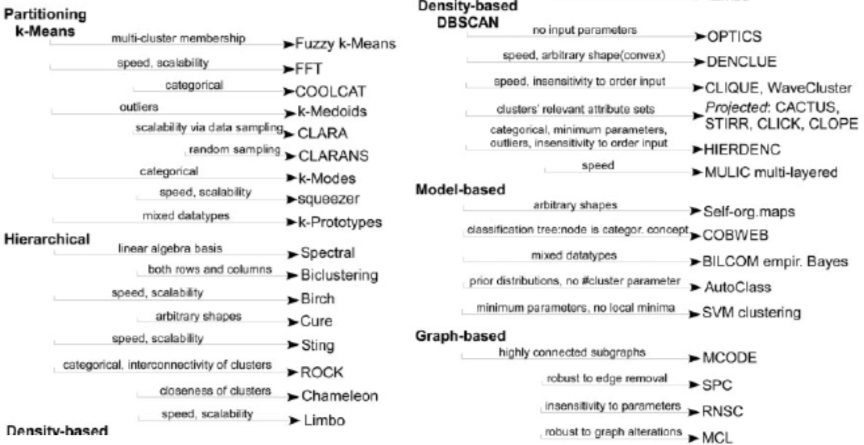
\includegraphics[scale = 0.5,angle = 0]{clustering_methods.png}
  \caption[Clustering Methods]{\normalsize{Clustering Methods}}
  \label{fig:Clustering}
  \end{figure}
  
  The methods are aimed around clustering, which we will further explore
  in the next section.
  
  \subsection{Clustering}\label{clustering}
  
  Clustering organizes a set of data items into groups so that items in
  the same group are similar to each other and different from those in
  other groups {[}Rec 1{]}. Clustering is helpful in finding patterns and
  similarities/differences between data points and groups; however it can
  be quite subjective, as we will discuss later on in the project.
  
  Clustering can be used in categorizing data based on non-spatial dat,
  
  \chapter{How to Cluster}\label{rmd-basics}
  
  There are many factors to consider when chosing a clustering algorithm,
  such as the application of the problem (what do you want to find out
  about this data?), quality vs speed trade off (size of data plays a
  role), characteristics of the data (i.e.~numeric distance measures),
  dimensionality (typically as dimension increases the time it takes to
  run the method increases and quality of the data clusters decrease), and
  outliers (some methods are very sensitive to outliers) {[}Rec 2{]}.
  
  \section{Types of Clustering:
  Partitioning}\label{types-of-clustering-partitioning}
  
  There are four main types of clustering: hierarchial, partitioning,
  density-based, and methods-based. We will now dive into the partioning
  clustering techinque.
  
  Partitioning cluster methods divide a set of data items into a number of
  non-overlapping clusters. A data item is typically assigned to a cluster
  based on a proximity or dissimilarity measure {[}Rec 2, p.~405{]}.
  
  Typically, there is a dataset with \emph{n} observations and the goal is
  to divide them into \emph{K} clusters so that an objective function is
  optimized (sum of square distances is minimized).
  
  The most common objective function is the sum of squared errors (SSE),
  where \(c_k\) is the centroid or mediod of the cluster \(C_k\).
  
  \[SSE(C)= \sum_{k=1}^K \sum_{x_{i}C_{k}} ||{x_i}- c_k||^2\]
  
  Partitioning clustering algorithms classifies the data into K groups by
  satisfying both that each group has at least one data point, and that
  each data point belongs to exactly one group. {[}Rec 5, p.~18{]}.
  
  \section{\texorpdfstring{How to Create Clusters: \emph{K}-Means vs
  \emph{K}-Medoids}{How to Create Clusters: K-Means vs K-Medoids}}\label{how-to-create-clusters-k-means-vs-k-medoids}
  
  \emph{K}-means algorithm and \emph{k}-medoid algorithm are two examples
  of partitioning algorithms. They both ise iterative processes to find
  \emph{K} clusters; however, they use different ways to represent these
  clusters.
  
  \subsection{\texorpdfstring{\emph{K}-Means (maybe don't include
  this)}{K-Means (maybe don't include this)}}\label{k-means-maybe-dont-include-this}
  
  \emph{K}-means algorithm represents its n observations in \emph{k}
  groups, with the center of the groups being the mean/average
  observation. The goal of the algorithm is to find k centroids, one for
  each cluster. In order to do this, we must minimize an \emph{objective
  function}, which is the squared error function for \emph{k} means. The
  objective function is:
  \[O= \sum_{j=1}^k \sum_{i=1}^j ||{{X_i^{(j)}- C_j}}||^2\]
  
  Where \(|{{X_i^{(j)}- C_j}}|\) is an indicator of the distance of the
  data points from their cluster centers.
  
  The steps of the algorithm are as follows:
  
  \begin{enumerate}
  \def\labelenumi{\arabic{enumi}.}
  \tightlist
  \item
    Choose K points in the space to represent the centroid. This works
    best if they are chosen to be far apart from eachother.
  \item
    Assign each object to the cluster with the closest centroid.
  \item
    When all of the clusters have been made, recalculate the positions of
    the K centroids.
  \item
    Repeat steps 2 and 3 until the centroids no longer move.
  \end{enumerate}
  
  This algorithm always terminates; however, it is sensitive both to
  outliers and to the initial randomly selected K cluster centers.
  Therefore, the algorithm should be run multiple times to reduce the
  effects from this sensitivity. {[}Rec 5, p.~18{]}.
  
  \subsection{\texorpdfstring{\emph{K}
  Medoids}{K Medoids}}\label{k-medoids}
  
  On the contrary, instead of taking the mean value of the objects in a
  cluster, the k-medoid method uses the most centrally located object in a
  cluster to be the cluster center {[}Rec 2{]}. This causes the method to
  be less sensitive to outliers, but also requires more time to run.
  
  Steps for K-medoids: 1. Initial guess for centers \(C_1\),
  \(C_2\),\ldots{} \(C_k\) (i.e.~randomly select k points from \(X_1\),
  \(X_2\),\ldots{} \(X_n\)) 2. Minimize over C: for each i= 1, 2,\ldots{}
  n, find the cluster center \(C_k\) closest to Xi and let C(i)=k. 3.
  Minimize over \(C_1\), \(C_2\),\ldots{} \(C_k\): for each k=1,\ldots{}
  K, \(C_k = X_k^*\), the medoid of points in cluster k. ie, the point Xi
  in the cluster k that minimizes \[\sum _{c(j)=k} ||{{X_j- X_i}}||^2\]
  
  \textbf{same steps as K-means except BLANK (p.~6 in Rec 2) }steps in Rec
  5, p.~19 for k-medoids
  
  Rec 5 p.~18-19 ***
  
  \begin{Shaded}
  \begin{Highlighting}[]
  \CommentTok{#How to insert a figure, make sure amherst.png is in main directory}
  
  \KeywordTok{label}\NormalTok{(}\DataTypeTok{path =} \StringTok{"clustering_pic.png"}\NormalTok{, }
        \DataTypeTok{caption =} \StringTok{"CLARANS searching for a better solution"}\NormalTok{, }
        \DataTypeTok{label =} \StringTok{"CLARANS"}\NormalTok{, }\DataTypeTok{type =} \StringTok{"figure"}\NormalTok{, }\DataTypeTok{scale=} \FloatTok{0.5}\NormalTok{)}
  \end{Highlighting}
  \end{Shaded}
  
  \begin{figure}[htbp]
  \centering
  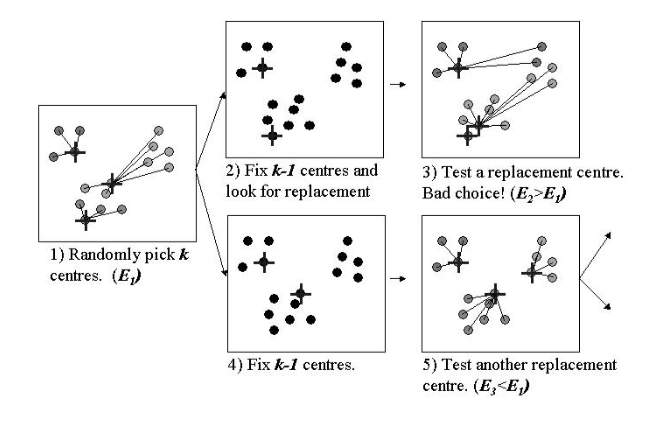
\includegraphics[scale = 0.5,angle = 0]{clustering_pic.png}
  \caption[CLARANS searching for a better solution]{\normalsize{CLARANS searching for a better solution}}
  \label{fig:CLARANS}
  \end{figure}
  
  \section{\texorpdfstring{How to Choose
  \emph{K}}{How to Choose K}}\label{how-to-choose-k}
  
  Many ways to choose \emph{k}, which is why these methods are so
  subjective.
  
  I will describe two of the many ways to determine K, both of which use
  visuals to determine what value of k is appropriate for the data. The
  elbow method and silhouette method are common ways to find K when using
  the \emph{K} means and \emph{K} medoids algorithms.
  
  \subsection{Elbow Method}\label{elbow-method}
  
  To start, the elbow method looks at the total within-cluster sum of
  squares (WSS) and determines when there are enough clusters so that the
  next cluster does not improve the total WSS very much. This would be the
  appropriate \emph{K}.
  
  The steps for this algorithm are as follows:
  
  \begin{enumerate}
  \def\labelenumi{\arabic{enumi}.}
  \tightlist
  \item
    Compute the clustering algorithm for different values of k (i.e.~k
    from 1 to 10).
  \item
    For each k, calculate the total WSS.
  \item
    Plot the curve of the total WSSs according to the number of clusters
    (k).
  \item
    The location of the bend in the plot is generally considered an
    indicator for the appropriate number of clusters.
  \end{enumerate}
  
  \subsection{Silhouette Method}\label{silhouette-method}
  
  The Silhouette Method focuses on the quality of clustering. A high
  average silhouette width indicates a good clustering (how well each
  object lies within its cluster).
  
  The steps of the Silhouette Algorithm are:
  
  \begin{enumerate}
  \def\labelenumi{\arabic{enumi}.}
  \tightlist
  \item
    Compute clustering algoritm for different values of k (i.e.~k from 1
    to 10).
  \item
    For each k, calculate the average silhouette of observations.
  \item
    Plot the curve of the average silhouettes according to the number of
    clusters (k).
  \item
    The location of the maximum is considered the appropriate number of
    clusters.
  \end{enumerate}
  
  --\textgreater{} datanovia website
  
  \chapter{Spatial Clustering Methods}\label{typeset-equ}
  
  \section{PAM}\label{pam}
  
  Partitioning Around Medoids (PAM) is the most commonly used type of
  k-medoid clustering (Kaufmann \& Rousseeuw, 1987).
  
  It iterates through all the k cluster centers and tries to replace the
  center with one of the other objects (n-k possibilities). {[}rec 2{]}.
  For a replacement to occur, the squared error function must decrease (if
  it does not decrease, there is no replacement). The algorithm eventually
  terminates with a local optimum.
  
  The total complexity of PAM in one iteration is **formula:
  \[O(k(n-k)^2)\] (o= each non-medoid data point, \emph{k}= \# of cluster
  centers, \[(n-k)\] objects to compare to, and \[(n-k)\] operations for
  calculating E). This makes for a costly computation when n is large.
  Works best for n= 100, k=5.
  
  Explanation of PAM, REC 6, P. 146--\textgreater{} 4 cases, and algorithm
  Rec 6 bibliography (Ng \& Han, 2000)
  
  \section{CLARA}\label{clara}
  
  Because PAM does not scale well to large data sets, Clustering LARge
  Applications (CLARA) was developed to deal with larger data sets
  (Kaufmann \& Rousseeuw, 1990).
  
  CLARA is a sampling based method, meaning a sample of the data is used
  to represent the entire data set. Medoids are chosen from this sample
  data using PAM and then ``the average dissimilarity is computed using
  the whole dataset'' (**don't know what ``average dissimilarity'' means
  or how it is calculated). If a new set of medoids gives a lower
  dissimilarity than a previous best solution, then the best solution is
  replaced with a new set of medoids {[}Rec 2, p.~7{]}.
  
  *PAM on samples
  
  \url{https://www.coursera.org/lecture/cluster-analysis/3-4-the-k-medoids-clustering-method-nJ0Sb}
  
  \section{CLARANS}\label{clarans}
  
  (Ng \& Han, 1994)
  
  *Randomized re-sampling, ensuring efficiency and quality
  
  \chapter{Example}\label{typeset-equ}
  
  \begin{Shaded}
  \begin{Highlighting}[]
  \CommentTok{#loading in packages}
  \KeywordTok{library}\NormalTok{(readr)}
  \KeywordTok{library}\NormalTok{(factoextra)}
  \end{Highlighting}
  \end{Shaded}
  
  \begin{verbatim}
  Welcome! Related Books: `Practical Guide To Cluster Analysis in R` at https://goo.gl/13EFCZ
  \end{verbatim}
  
  \begin{Shaded}
  \begin{Highlighting}[]
  \KeywordTok{library}\NormalTok{(NbClust)}
  \KeywordTok{library}\NormalTok{(ggplot2)}
  \KeywordTok{library}\NormalTok{(cluster)}
  \KeywordTok{library}\NormalTok{(GGally)}
  \end{Highlighting}
  \end{Shaded}
  
  \begin{verbatim}
  
  Attaching package: 'GGally'
  \end{verbatim}
  
  \begin{verbatim}
  The following object is masked from 'package:dplyr':
  
      nasa
  \end{verbatim}
  
  \section{Exploring the Data}\label{exploring-the-data}
  
  Data came from Stat 495 final project. (use info from project\ldots{}).
  Needed a sample of 1000\ldots{}
  
  Importing the data:
  
  \begin{Shaded}
  \begin{Highlighting}[]
  \CommentTok{#using data from final stat 495 project}
  \CommentTok{#library(readr)}
  \NormalTok{data_subset <-}\StringTok{ }\KeywordTok{read_csv}\NormalTok{(}\StringTok{"CopyOfdata_subset.csv"}\NormalTok{)}
  \end{Highlighting}
  \end{Shaded}
  
  \begin{verbatim}
  Parsed with column specification:
  cols(
    .default = col_double(),
    geo_name = col_character(),
    geo = col_character(),
    zip = col_character(),
    TRI.ID = col_character(),
    County.x = col_character(),
    County.y = col_character()
  )
  \end{verbatim}
  
  \begin{verbatim}
  See spec(...) for full column specifications.
  \end{verbatim}
  
  \begin{Shaded}
  \begin{Highlighting}[]
  \KeywordTok{set.seed}\NormalTok{(}\DecValTok{1}\NormalTok{)}
  \CommentTok{#getting a sample of 1000 observations}
  \NormalTok{mysample <-}\StringTok{ }\NormalTok{data_subset[}\KeywordTok{sample}\NormalTok{(}\DecValTok{1}\OperatorTok{:}\KeywordTok{nrow}\NormalTok{(data_subset), }\DecValTok{1000}\NormalTok{,}
     \DataTypeTok{replace=}\OtherTok{FALSE}\NormalTok{),]}
  \end{Highlighting}
  \end{Shaded}
  
  Picking variables to focus on--\textgreater{} expanding conclusions from
  Stat 495 project
  
  \begin{Shaded}
  \begin{Highlighting}[]
  \CommentTok{#only keeping the variables I want to look at}
  \NormalTok{myvars <-}\StringTok{ }\KeywordTok{c}\NormalTok{(}\StringTok{"Latitude_tri"}\NormalTok{, }\StringTok{"Longitude_tri"}\NormalTok{, }\StringTok{"poor_or_fair_health"}\NormalTok{, }\StringTok{"poor_physical_health_days"}\NormalTok{, }\StringTok{"physical_inactivity"}\NormalTok{, }\StringTok{"adult_obesity"}\NormalTok{)}
  \NormalTok{smallsample <-}\StringTok{ }\NormalTok{mysample[myvars]}
  \end{Highlighting}
  \end{Shaded}
  
  \section{Applying CLARA}\label{applying-clara}
  
  Step 1: finding k
  
  \begin{Shaded}
  \begin{Highlighting}[]
  \CommentTok{#finding k with project data, using Elbow Method}
  \CommentTok{#pkgs <- c("factoextra",  "NbClust")}
  \CommentTok{#install.packages(pkgs)}
  
  \CommentTok{#library(factoextra)}
  \CommentTok{#library(NbClust)}
  \CommentTok{#library(ggplot2)}
  \NormalTok{new<-}\StringTok{ }\KeywordTok{na.omit}\NormalTok{(smallsample)}
  \CommentTok{# Elbow method}
  \KeywordTok{fviz_nbclust}\NormalTok{(new, kmeans, }\DataTypeTok{method =} \StringTok{"wss"}\NormalTok{) }\OperatorTok{+}
  \StringTok{    }\KeywordTok{geom_vline}\NormalTok{(}\DataTypeTok{xintercept =} \DecValTok{4}\NormalTok{, }\DataTypeTok{linetype =} \DecValTok{2}\NormalTok{)}\OperatorTok{+}
  \StringTok{  }\KeywordTok{labs}\NormalTok{(}\DataTypeTok{subtitle =} \StringTok{"Elbow method"}\NormalTok{)}
  \end{Highlighting}
  \end{Shaded}
  
  \begin{center}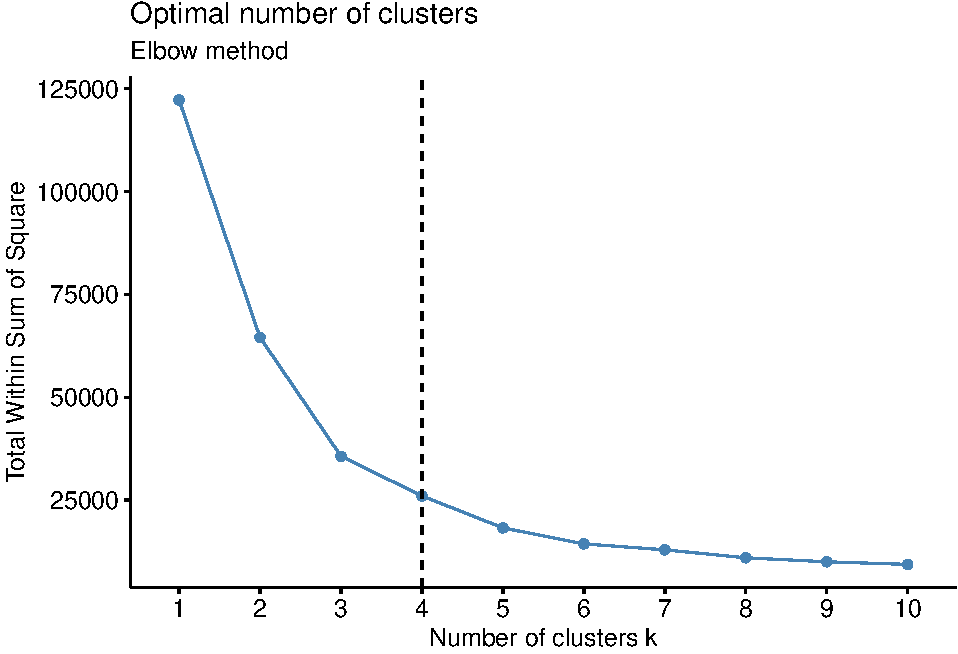
\includegraphics{Comps_Proj_files/figure-latex/unnamed-chunk-4-1} \end{center}
  
  Step 2: Run CLARA function
  
  \begin{Shaded}
  \begin{Highlighting}[]
  \CommentTok{#new<- na.omit(smallsample)}
  \CommentTok{#library(cluster)}
  \NormalTok{## run CLARA}
  \NormalTok{clarasamp <-}\StringTok{ }\KeywordTok{clara}\NormalTok{(new[}\DecValTok{1}\OperatorTok{:}\DecValTok{6}\NormalTok{], }\DecValTok{4}\NormalTok{)}
  \end{Highlighting}
  \end{Shaded}
  
  \begin{Shaded}
  \begin{Highlighting}[]
  \NormalTok{## print components of clarax}
  \KeywordTok{print}\NormalTok{(clarasamp)}
  \end{Highlighting}
  \end{Shaded}
  
  \begin{verbatim}
  Call:    clara(x = new[1:6], k = 4) 
  Medoids:
       Latitude_tri Longitude_tri poor_or_fair_health
  [1,]      38.6364      -83.6929               0.200
  [2,]      40.3973      -75.9357               0.165
  [3,]      36.1335      -96.0532               0.196
  [4,]      45.4342     -123.0000               0.110
       poor_physical_health_days physical_inactivity adult_obesity
  [1,]                       4.4               0.299         0.283
  [2,]                       3.7               0.245         0.308
  [3,]                       4.6               0.353         0.355
  [4,]                       3.3               0.137         0.244
  Objective function:  4.691022
  Clustering vector:   int [1:925] 1 2 1 3 1 3 1 1 1 1 1 3 1 2 1 3 3 3 ...
  Cluster sizes:           453 195 230 47 
  Best sample:
   [1]   5  11  24  86 139 149 162 175 177 192 208 224 242 285 306 311 316
  [18] 353 361 370 389 400 404 410 429 468 471 478 489 506 589 679 691 703
  [35] 719 726 736 741 800 811 815 818 877 882 883 895 902 918
  
  Available components:
   [1] "sample"     "medoids"    "i.med"      "clustering" "objective" 
   [6] "clusinfo"   "diss"       "call"       "silinfo"    "data"      
  \end{verbatim}
  
  \begin{Shaded}
  \begin{Highlighting}[]
  \KeywordTok{summary}\NormalTok{(clarasamp)}
  \end{Highlighting}
  \end{Shaded}
  
  \begin{verbatim}
  Object of class 'clara' from call:
   clara(x = new[1:6], k = 4) 
  Medoids:
       Latitude_tri Longitude_tri poor_or_fair_health
  [1,]      38.6364      -83.6929               0.200
  [2,]      40.3973      -75.9357               0.165
  [3,]      36.1335      -96.0532               0.196
  [4,]      45.4342     -123.0000               0.110
       poor_physical_health_days physical_inactivity adult_obesity
  [1,]                       4.4               0.299         0.283
  [2,]                       3.7               0.245         0.308
  [3,]                       4.6               0.353         0.355
  [4,]                       3.3               0.137         0.244
  Objective function:   4.691022 
  Numerical information per cluster:
       size  max_diss  av_diss isolation
  [1,]  453 13.228882 4.578281  1.656594
  [2,]  195  8.392191 2.971767  1.050917
  [3,]  230 14.554453 6.249473  1.153918
  [4,]   47 42.497226 5.284278  1.489171
  Average silhouette width per cluster:
  [1] 0.2863797 0.6457187 0.4655863 0.9673973
  Average silhouette width of best sample: 0.4306859 
  
  Best sample:
   [1]   5  11  24  86 139 149 162 175 177 192 208 224 242 285 306 311 316
  [18] 353 361 370 389 400 404 410 429 468 471 478 489 506 589 679 691 703
  [35] 719 726 736 741 800 811 815 818 877 882 883 895 902 918
  Clustering vector:
    [1] 1 2 1 3 1 3 1 1 1 1 1 3 1 2 1 3 3 3 3 2 1 3 2 1 1 3 3 2 2 1 1 2 3 1 3
   [36] 1 1 1 3 3 1 1 1 1 1 1 1 1 1 2 1 1 3 1 1 1 1 4 1 1 1 1 2 2 3 3 1 2 1 3
   [71] 1 1 3 3 1 3 1 4 1 2 1 2 4 1 1 3 1 2 4 3 3 3 1 1 3 4 4 1 2 2 1 2 3 3 1
  [106] 1 1 3 3 4 1 3 3 4 2 1 2 3 2 3 2 2 1 3 1 2 1 1 1 3 2 4 1 2 1 1 2 1 3 3
  [141] 1 2 1 1 1 1 2 1 1 2 2 1 1 3 3 1 3 1 3 1 3 1 1 2 1 3 1 4 3 1 1 3 1 3 3
  [176] 1 3 1 1 4 2 1 1 1 1 2 1 1 3 1 1 3 2 1 2 3 3 2 1 1 1 2 1 3 2 1 2 1 1 1
  [211] 1 1 1 2 1 3 4 2 4 3 1 1 3 2 1 1 3 4 3 2 2 1 1 1 3 3 1 1 3 1 1 2 1 2 3
  [246] 2 1 1 3 1 1 3 4 2 1 1 2 3 1 2 1 1 1 3 1 4 2 3 2 1 3 2 2 3 1 1 3 2 1 3
  [281] 1 1 3 3 1 1 3 1 2 2 3 1 1 3 1 2 1 1 1 1 1 3 1 1 1 1 3 3 1 3 1 1 3 1 1
  [316] 3 1 2 1 1 1 3 2 3 1 1 3 1 1 4 2 1 1 1 3 1 2 1 2 2 1 3 1 1 3 3 4 3 1 1
  [351] 1 1 1 1 1 3 1 3 1 1 1 3 3 1 2 1 3 1 2 3 1 3 3 2 2 2 1 1 3 2 3 3 3 1 1
  [386] 1 1 2 1 3 1 1 2 1 2 2 1 3 3 2 1 4 2 2 1 1 1 1 1 1 3 1 1 1 1 1 2 1 3 1
  [421] 3 3 2 3 1 2 1 3 2 1 1 1 1 4 4 1 1 3 1 2 1 1 1 3 1 2 1 1 2 1 3 1 1 2 4
  [456] 1 1 2 1 1 1 2 1 1 4 3 1 1 4 4 1 1 3 1 4 1 1 1 1 3 4 2 1 1 1 1 2 2 3 1
  [491] 2 3 1 3 3 1 2 2 2 2 1 2 2 3 1 1 2 3 2 1 1 2 3 2 3 3 2 2 2 3 2 1 3 2 3
  [526] 3 3 1 4 1 1 2 2 2 1 3 2 1 1 1 3 4 1 1 3 1 1 2 3 1 2 1 3 1 1 3 2 3 3 3
  [561] 1 2 1 2 1 3 2 3 1 4 1 1 3 3 2 1 1 3 2 2 1 1 2 1 2 1 1 1 1 3 2 1 3 4 1
  [596] 3 1 1 2 1 3 2 3 4 1 3 1 1 1 4 3 1 2 1 1 3 4 2 1 2 3 2 1 2 3 1 1 2 1 2
  [631] 1 1 4 3 1 2 3 1 1 3 1 4 3 1 1 1 2 2 3 2 1 1 1 2 1 1 1 2 3 1 3 1 1 3 1
  [666] 1 1 1 3 1 2 1 3 1 1 1 1 1 2 2 3 1 2 3 2 2 1 1 2 2 3 2 1 1 1 2 1 3 3 1
  [701] 1 1 1 4 2 1 3 1 1 2 4 3 1 1 1 3 3 1 1 1 1 3 1 1 2 4 2 3 1 1 1 3 1 1 3
  [736] 1 2 1 2 3 2 2 2 1 3 3 3 1 1 1 2 3 3 3 1 3 3 2 1 2 3 3 1 2 4 2 1 1 3 1
  [771] 2 1 1 1 3 1 3 3 1 1 3 3 1 3 1 2 1 1 3 1 4 1 1 1 1 3 2 2 2 4 1 3 3 1 1
  [806] 1 3 1 1 1 2 1 1 1 2 2 2 1 1 2 1 3 3 3 3 1 3 2 4 2 1 2 3 1 1 3 2 1 1 4
  [841] 2 2 2 2 2 1 3 1 2 1 2 4 3 3 1 1 3 1 1 1 1 1 2 3 3 2 4 1 2 1 1 1 1 2 1
  [876] 1 3 1 1 1 3 3 1 1 1 3 1 1 3 1 1 3 1 3 1 3 2 2 2 3 1 2 2 2 1 1 4 1 2 1
  [911] 3 1 3 2 3 3 1 1 2 1 3 1 1 3 1
  
  Silhouette plot information for best sample:
      cluster neighbor   sil_width
  11        1        2  0.51160188
  703       1        2  0.50784463
  149       1        3  0.50590891
  208       1        2  0.48693148
  162       1        3  0.47468187
  471       1        2  0.44956360
  410       1        2  0.42362707
  389       1        2  0.42157038
  5         1        2  0.41457596
  719       1        2  0.41289559
  468       1        2  0.37020730
  361       1        2  0.35061984
  306       1        2  0.34569720
  285       1        2  0.34506744
  818       1        3  0.30770633
  506       1        3  0.21671937
  589       1        2  0.20444489
  918       1        2  0.19851903
  736       1        3  0.18549695
  478       1        2  0.16554915
  24        1        2  0.15565598
  311       1        2  0.04768370
  353       1        3  0.03173421
  883       1        2 -0.12930919
  895       1        2 -0.24550081
  224       2        1  0.76643863
  679       2        1  0.75957431
  902       2        1  0.74802681
  404       2        1  0.74508892
  242       2        1  0.73417881
  400       2        1  0.73283435
  741       2        1  0.61737358
  811       2        1  0.47833894
  815       2        1  0.43844208
  429       2        1  0.43689016
  691       3        1  0.62256512
  370       3        1  0.62175433
  489       3        1  0.61988506
  882       3        1  0.60671130
  139       3        1  0.58178390
  177       3        1  0.55053388
  175       3        1  0.43464488
  86        3        1  0.29525285
  192       3        1  0.28445790
  316       3        1  0.27777790
  877       3        1  0.22608234
  800       4        3  0.96743579
  726       4        3  0.96735884
  
  1128 dissimilarities, summarized :
     Min. 1st Qu.  Median    Mean 3rd Qu.    Max. 
   0.0507  6.3776 10.6340 12.8320 15.7130 51.8530 
  Metric :  euclidean 
  Number of objects : 48
  
  Available components:
   [1] "sample"     "medoids"    "i.med"      "clustering" "objective" 
   [6] "clusinfo"   "diss"       "call"       "silinfo"    "data"      
  \end{verbatim}
  
  \begin{Shaded}
  \begin{Highlighting}[]
  \NormalTok{## plot clusters}
  \KeywordTok{plot}\NormalTok{(new, }\DataTypeTok{col =}\NormalTok{ clarasamp}\OperatorTok{$}\NormalTok{cluster)}
  \NormalTok{## plot centers}
  \KeywordTok{points}\NormalTok{(clarasamp}\OperatorTok{$}\NormalTok{centers, }\DataTypeTok{col =} \DecValTok{1}\OperatorTok{:}\DecValTok{2}\NormalTok{, }\DataTypeTok{pch =} \DecValTok{8}\NormalTok{)}
  \end{Highlighting}
  \end{Shaded}
  
  \begin{center}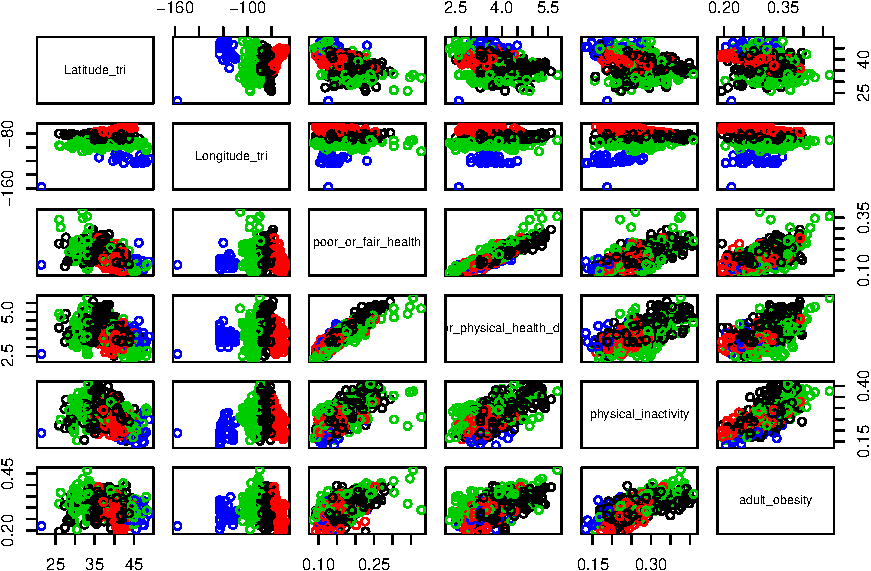
\includegraphics{Comps_Proj_files/figure-latex/unnamed-chunk-7-1} \end{center}
  
  \begin{Shaded}
  \begin{Highlighting}[]
  \CommentTok{#plotting clara}
  \NormalTok{factoextra}\OperatorTok{::}\KeywordTok{fviz_cluster}\NormalTok{(clarasamp)}
  \end{Highlighting}
  \end{Shaded}
  
  \begin{center}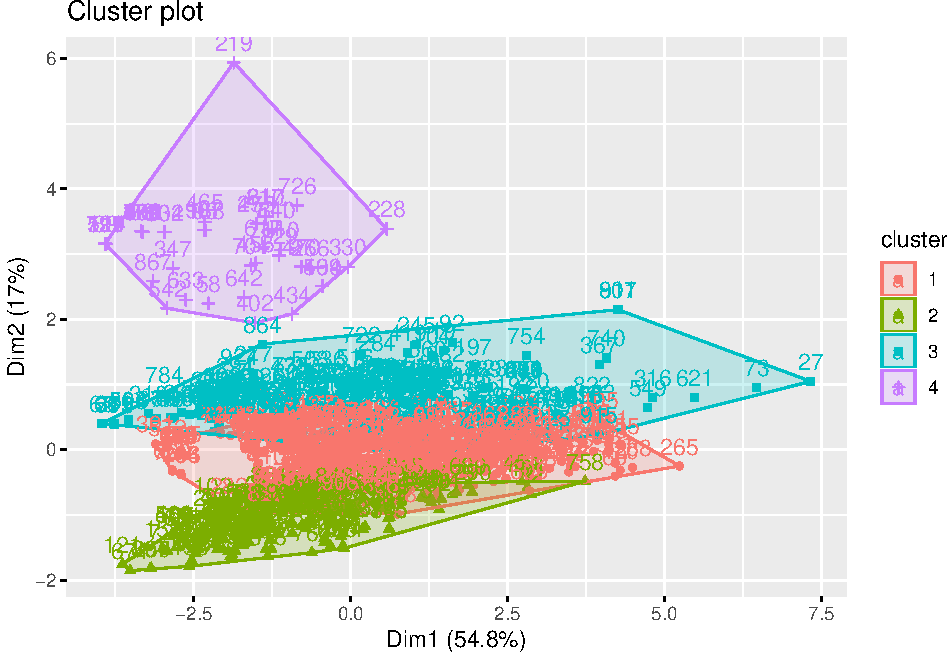
\includegraphics{Comps_Proj_files/figure-latex/unnamed-chunk-8-1} \end{center}
  
  \section{Evaluation of CLARA}\label{evaluation-of-clara}
  
  \subsection{Model to Predict Cluster}\label{model-to-predict-cluster}
  
  First, had to include a cluster variable in the original data set, using
  the data provided by the CLARA function.
  
  \begin{Shaded}
  \begin{Highlighting}[]
  \CommentTok{#adding each data point's cluster #}
  \NormalTok{cluster<-}\StringTok{ }\NormalTok{clarasamp}\OperatorTok{$}\NormalTok{clustering}
  \NormalTok{cluster_data<-}\StringTok{ }\KeywordTok{cbind}\NormalTok{(new, cluster)}
  \end{Highlighting}
  \end{Shaded}
  
  \begin{Shaded}
  \begin{Highlighting}[]
  \NormalTok{kitchen_sink<-}\StringTok{ }\KeywordTok{lm}\NormalTok{(cluster}\OperatorTok{~}\NormalTok{., }\DataTypeTok{data=}\NormalTok{cluster_data)}
  \KeywordTok{summary}\NormalTok{(kitchen_sink)}
  \end{Highlighting}
  \end{Shaded}
  
  \begin{verbatim}
  
  Call:
  lm(formula = cluster ~ ., data = cluster_data)
  
  Residuals:
      Min      1Q  Median      3Q     Max 
  -2.3742 -0.6013  0.0600  0.6334  1.6092 
  
  Coefficients:
                             Estimate Std. Error t value Pr(>|t|)    
  (Intercept)               -1.373221   0.386769  -3.550 0.000404 ***
  Latitude_tri               0.004183   0.006661   0.628 0.530140    
  Longitude_tri             -0.055900   0.002255 -24.786  < 2e-16 ***
  poor_or_fair_health        8.194392   1.457716   5.621 2.51e-08 ***
  poor_physical_health_days -0.913749   0.090846 -10.058  < 2e-16 ***
  physical_inactivity        1.395680   0.751308   1.858 0.063536 .  
  adult_obesity             -0.419444   0.839018  -0.500 0.617249    
  ---
  Signif. codes:  0 '***' 0.001 '**' 0.01 '*' 0.05 '.' 0.1 ' ' 1
  
  Residual standard error: 0.6984 on 918 degrees of freedom
  Multiple R-squared:  0.4751,    Adjusted R-squared:  0.4717 
  F-statistic: 138.5 on 6 and 918 DF,  p-value: < 2.2e-16
  \end{verbatim}
  
  \begin{Shaded}
  \begin{Highlighting}[]
  \CommentTok{#taking out lat and long}
  \NormalTok{vars <-}\StringTok{ }\KeywordTok{names}\NormalTok{(cluster_data) }\OperatorTok\StringTok{ }\KeywordTok{c}\NormalTok{(}\StringTok{"Latitude_tri"}\NormalTok{, }\StringTok{"Longitude_tri"}\NormalTok{)}
  \NormalTok{cluster_data_new <-}\StringTok{ }\NormalTok{cluster_data[}\OperatorTok{!}\NormalTok{vars]}
  
  \KeywordTok{ggpairs}\NormalTok{(cluster_data_new)}
  \end{Highlighting}
  \end{Shaded}
  
  \begin{center}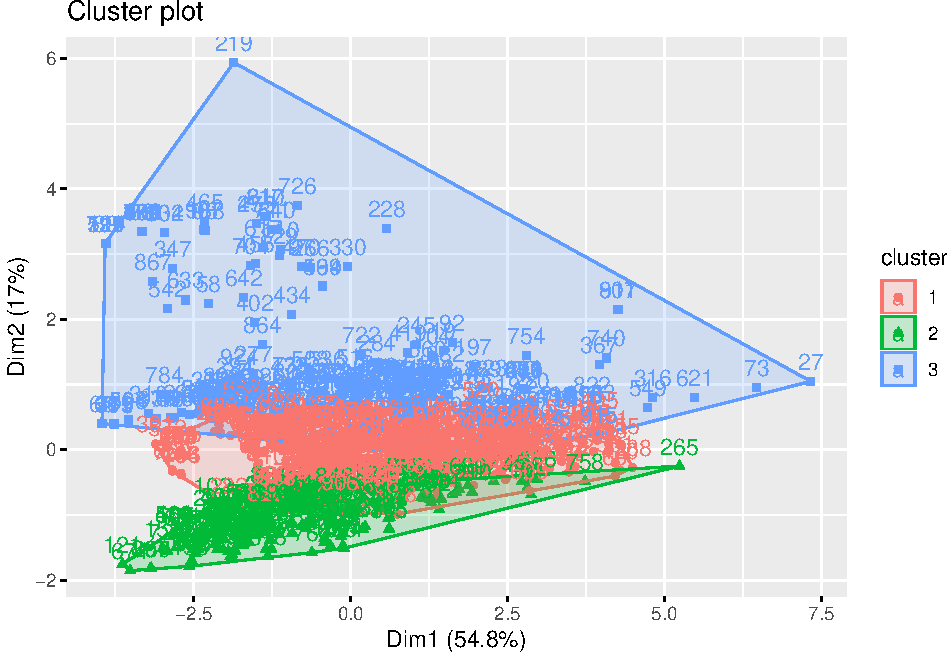
\includegraphics{Comps_Proj_files/figure-latex/unnamed-chunk-10-1} \end{center}
  
  \begin{Shaded}
  \begin{Highlighting}[]
  \NormalTok{fun1<-}\StringTok{ }\KeywordTok{lm}\NormalTok{(cluster}\OperatorTok{~}\StringTok{ }\NormalTok{poor_physical_health_days, }\DataTypeTok{data=}\NormalTok{ cluster_data_new)}
  \KeywordTok{summary}\NormalTok{(fun1)}
  \end{Highlighting}
  \end{Shaded}
  
  \begin{verbatim}
  
  Call:
  lm(formula = cluster ~ poor_physical_health_days, data = cluster_data_new)
  
  Residuals:
      Min      1Q  Median      3Q     Max 
  -1.3539 -0.8070 -0.1857  0.8144  2.4875 
  
  Coefficients:
                            Estimate Std. Error t value Pr(>|t|)    
  (Intercept)                3.40573    0.19278  17.667  < 2e-16 ***
  poor_physical_health_days -0.42072    0.05183  -8.118 1.51e-15 ***
  ---
  Signif. codes:  0 '***' 0.001 '**' 0.01 '*' 0.05 '.' 0.1 ' ' 1
  
  Residual standard error: 0.9288 on 923 degrees of freedom
  Multiple R-squared:  0.06664,   Adjusted R-squared:  0.06563 
  F-statistic:  65.9 on 1 and 923 DF,  p-value: 1.509e-15
  \end{verbatim}
  
  \chapter*{Conclusion}\label{conclusion}
  \addcontentsline{toc}{chapter}{Conclusion}
  
  \setcounter{chapter}{4} \setcounter{section}{0}
  
  If we don't want Conclusion to have a chapter number next to it, we can
  add the \texttt{\{.unnumbered\}} attribute. This has an unintended
  consequence of the sections being labeled as 3.6 for example though
  instead of 4.1. The \LaTeX~commands immediately following the Conclusion
  declaration get things back on track.
  
  \subsubsection{More info}\label{more-info}
  
  And here's some other random info: the first paragraph after a chapter
  title or section head \emph{shouldn't be} indented, because indents are
  to tell the reader that you're starting a new paragraph. Since that's
  obvious after a chapter or section title, proper typesetting doesn't add
  an indent there.
  
  \appendix
  
  \singlespacing
  
  \chapter{The First Appendix}\label{the-first-appendix}
  
  This first appendix includes all of the R chunks of code that were
  hidden throughout the document (using the \texttt{include\ =\ FALSE}
  chunk tag) to help with readibility and/or setup.
  
  \subsubsection{In the main Rmd file:}\label{in-the-main-rmd-file}
  
  \begin{Shaded}
  \begin{Highlighting}[]
  \CommentTok{# This chunk ensures that the acstats package is}
  \CommentTok{# installed and loaded. This acstats package includes}
  \CommentTok{# the template files for the thesis and also two functions}
  \CommentTok{# used for labeling and referencing}
  \ControlFlowTok{if}\NormalTok{(}\OperatorTok{!}\KeywordTok{require}\NormalTok{(devtools))}
    \KeywordTok{install.packages}\NormalTok{(}\StringTok{"devtools"}\NormalTok{, }\DataTypeTok{repos =} \StringTok{"http://cran.rstudio.com"}\NormalTok{)}
  \ControlFlowTok{if}\NormalTok{(}\OperatorTok{!}\KeywordTok{require}\NormalTok{(acstats))\{}
    \KeywordTok{library}\NormalTok{(devtools)}
  \NormalTok{  devtools}\OperatorTok{::}\KeywordTok{install_github}\NormalTok{(}\StringTok{"Amherst-Statistics/acstats"}\NormalTok{)}
  \NormalTok{\}}
  \KeywordTok{library}\NormalTok{(acstats)}
  \end{Highlighting}
  \end{Shaded}
  
  \subsubsection{\texorpdfstring{In
  \protect\hyperlink{ref_labels}{}:}{In :}}\label{in}
  
  \begin{Shaded}
  \begin{Highlighting}[]
  \CommentTok{# This chunk ensures that the acstats package is}
  \CommentTok{# installed and loaded. This acstats package includes}
  \CommentTok{# the template files for the thesis and also two functions}
  \CommentTok{# used for labeling and referencing}
  \ControlFlowTok{if}\NormalTok{(}\OperatorTok{!}\KeywordTok{require}\NormalTok{(devtools))}
    \KeywordTok{install.packages}\NormalTok{(}\StringTok{"devtools"}\NormalTok{, }\DataTypeTok{repos =} \StringTok{"http://cran.rstudio.com"}\NormalTok{)}
  \ControlFlowTok{if}\NormalTok{(}\OperatorTok{!}\KeywordTok{require}\NormalTok{(dplyr))}
      \KeywordTok{install.packages}\NormalTok{(}\StringTok{"dplyr"}\NormalTok{, }\DataTypeTok{repos =} \StringTok{"http://cran.rstudio.com"}\NormalTok{)}
  \ControlFlowTok{if}\NormalTok{(}\OperatorTok{!}\KeywordTok{require}\NormalTok{(ggplot2))}
      \KeywordTok{install.packages}\NormalTok{(}\StringTok{"ggplot2"}\NormalTok{, }\DataTypeTok{repos =} \StringTok{"http://cran.rstudio.com"}\NormalTok{)}
  \ControlFlowTok{if}\NormalTok{(}\OperatorTok{!}\KeywordTok{require}\NormalTok{(acstats))\{}
    \KeywordTok{library}\NormalTok{(devtools)}
  \NormalTok{  devtools}\OperatorTok{::}\KeywordTok{install_github}\NormalTok{(}\StringTok{"Amherst-Statistics/acstats"}\NormalTok{)}
  \NormalTok{\}}
  \end{Highlighting}
  \end{Shaded}
  
  \chapter{The Second Appendix, for
  Fun}\label{the-second-appendix-for-fun}
  
  \backmatter
  
  \chapter{References}\label{references}
  
  \noindent
  
  \setlength{\parindent}{-0.20in} \setlength{\leftskip}{0.20in}
  \setlength{\parskip}{8pt}
  
  \hypertarget{refs}{}
  \hypertarget{ref-angel2001}{}
  Angel, E. (2001a). \emph{Batch-file computer graphics : A bottom-up
  approach with quicktime}. Boston, MA: Wesley Addison Longman.
  
  \hypertarget{ref-angel2002a}{}
  Angel, E. (2001b). \emph{Test second book by angel}. Boston, MA: Wesley
  Addison Longman.
  
  \hypertarget{ref-ng1994}{}
  Ng, R. T., \& Han, J. (2000). \emph{Efficient and effective clustering
  methods for spatial data mining}. San Francisco, CA: Morgan Kaufmann
  Publishers Inc.


  % Index?

\end{document}

